
\section{Introdução}
\label{sec:introducao_scheme}

Como discutido no capítulo anterior, a linguagem \textit{Scheme} mantém
características de minimalismo e simplicidade conceitual que a tornaram
bastante populares como ambiente de estudo de conceitos e implementações de
linguagens de programação além de ser utilizada em diversas instituições de
ensino como linguagem inicial para aprendizado de conceitos de computação e
programação.

Praticamente todas estas características, no entanto, são meros acidentes no
processo de desenvolvimento da linguagem. Ela foi desenvolvida por Gerald Jay
Sussman e Guy L. Steele Jr com o objetivo de  criar um dialeto Lisp simples
para mapear e melhor compreender o modelo de computação chamado ``\textit{Actor
Model}''. Este modelo foi proposto por Carl Hewitt \textit{et al}, em seu paper
``\textit{A Universal Modular Actor Formalism for Artificial Intelligence}''.
Esta implementação inicial, publicada ao longo de diversos memorandos entre
1975 e 1980, resultou na linguagem de programação \textit{Scheme}.\cite{first-report}

Como resultado deste empreendimento, Sussman e Steele acabaram por descobrir
que o modelo proposto por Hewitt podia ser diretamente traduzido para o modelo
de computação já bastante conhecido à época chamada Cálculo Lambda. Perceberam
também que um dialeto Lisp baseado no Cálculo Lambda poderia ser criado com
pequenas alterações nos modelos computacionais utilizados pelos dialetos Lisp
utilizados na época. Chegaram à conclusão que um dialeto Lisp poderia ser
criado para representar o \textit{Actor Model} bastando que se passasse a
utilizar uma estratégia de escopo léxico (em contraste com o escopo dinâmico
utilizado por todos os dialetos Lisp da época) e que o conceito de
\textit{Continuações} fosse exposto como objetos de primeira classe.

A criação deste dialeto Lisp, então chamado \textit{Schemer} como uma
brincadeira em relação ao nome de outras duas linguagens criadas por times
próximos (\textit{Planner} e \textit{Conniver}), baseado mais fortemente no
modelo do Cálculo Lambda, criou uma forma prática para que estudos teóricos
feitos sobre a base do Cálculo Lambda tivessem uma materialização prática na
forma de uma linguagem de programação em que poderiam ser experimentados. Esta
acabou por se tornar uma ótima plataforma de experimentação\cite{first-report}.

A seguir, é descrito um subconjunto das funcionalidades de \textit{Scheme} de forma a
familiarizar o leitor com a linguagem e facilitar a compreensão da subsequente
discussão de sua implementação e as estratégias utilizadas.

\section{Descrição da linguagem e suas funcionalidades}
\label{sec:funcionalidades}

Variáveis em \textit{Scheme} não possuem tipo. O tipo é uma propriedade do
valor armazenado na variável, com a checagem dos tipos feita em tempo de
execução, não havendo verificação estática desta característica. A linguagem
vem equipada com um conjunto modesto de tipos e permite ao programador criar
seus próprios tipos disjuntos dos tipos existentes.

Além disso, não existe em \textit{Scheme} o conceito de classes, como em
linguagens orientadas a objeto, embora este conceito tenha sido diversas vezes
implementado em termos das primitivas da linguagem \cite{tinyclos}\cite{meroon3}\cite{scheme/objects}.

Seu caráter minimalista pode ser verificado na forma como primitivas que são
comuns em outras linguagens simplesmente não existem em \textit{Scheme}, sendo
substituídas por construções compostas de primitivas mais abrangentes.  Por
exemplo, no lugar de expressões de retorno, mecanismos de exceções ou
interrupções de estruturas de laço (como \textit{break} e \textit{continue}),
temos apenas as primitivas de obter a continuação atual e aplicar uma
continuação e formas sintáticas derivadas desta primitiva. Até mesmo as
estruturas de laço não são primitivas em \textit{Scheme}: são meros padrões de
utilização das primitivas de criar uma nova função e aplicação de funções.

A seguir são discutidas algumas características de \textit{Scheme} que a
diferenciam de grande parte das linguagens de uso geral em ampla utilização
atualmente ou que a diferenciam das linguagens anteriores da família
\textit{Lisp}.

\subsection{Eliminação de Chamadas Terminais}

Toda implementação de \textit{Scheme} é obrigada a realizar a eliminação dos
registros de ativação de chamadas a funções quandos estas funções estiverem 
na condição conhecida como uma ``chamada terminal'' (também conhecidas como 
\textit{tail-calls}): aplicações de função
nas quais o resultado da função chamada será, também, o resultado da função
chamadora.

Esta obrigação deriva da utilização de funções como estruturas de laço,
utilizando recursão: se a cada iteração for criado um novo registro de ativação
irrelevante, é possível que a memória de uma implementação arbitrária seja
esgotada por um laço longo o suficiente (por exemplo, esgotando a pilha
utilizada para manter a cadeia de chamadas). Como exemplo, o código a seguir
exibe uma função recursiva simples que retorna a soma de dois números naturais
utilizando apenas as operações de incremento e decremento.

\begin{lstlisting}[frame=none]
    (define (add op1 op2)
      (if (zero? op1)
        op2
        (add (dec op1) (inc op2))))
\end{lstlisting}

Esta função é obviamente recursiva, no entanto chamada recursiva aparece em uma
posição terminal. Na figura \ref{fig:tail-call-elimination} pode-se verificar
como seria o consumo de memória utilizado para armazenar os registros de
ativação em duas implementações hipotéticas com e sem eliminação de chamadas
terminais.

\begin{figure}[h!]
\centering
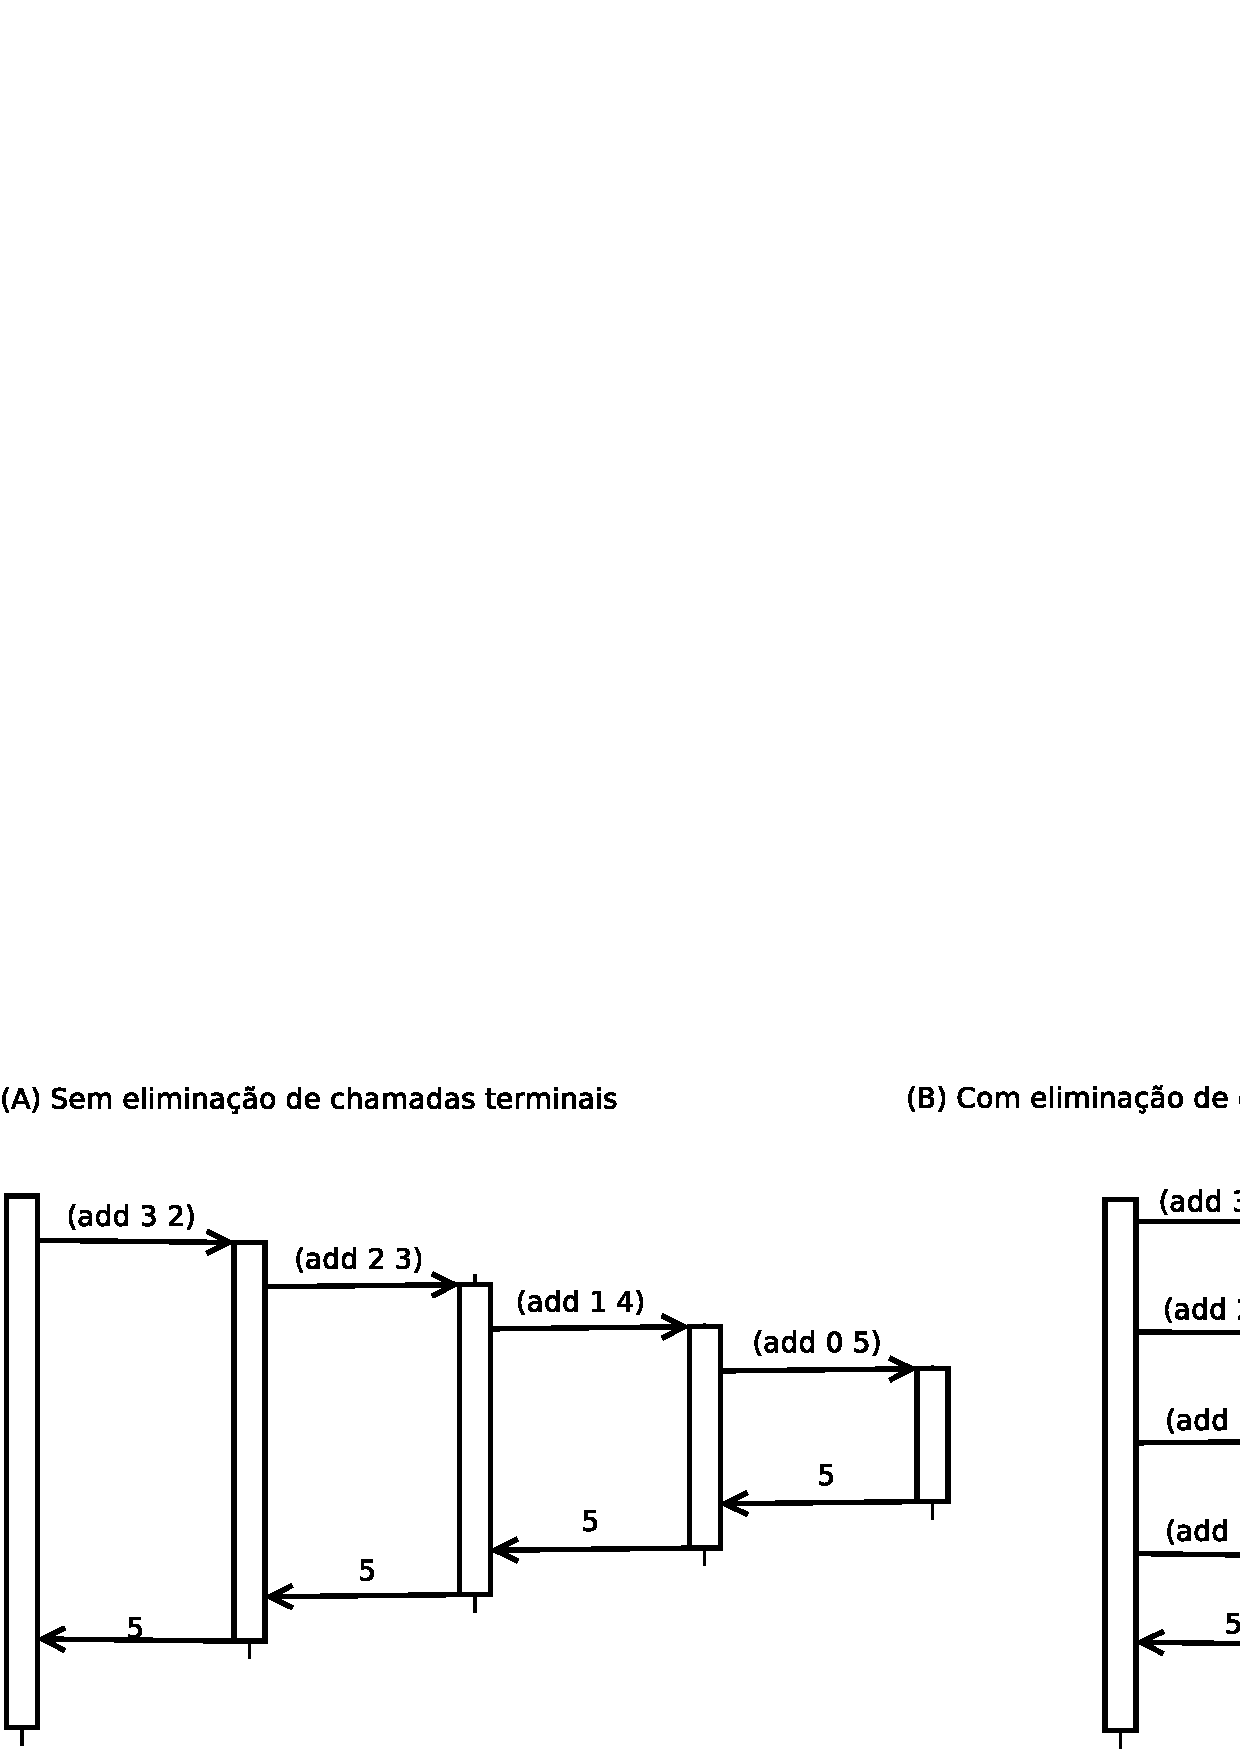
\includegraphics[width=0.9\textwidth]{../images/tail-call-elimination.pdf}
\caption{Tempo de vida de registros de ativação em relação a chamadas terminais}
\label{fig:tail-call-elimination}
\end{figure}

Quando uma implementação \textit{Scheme} se depara com uma aplicação de chamada
de função terminal, esta deve evitar criar um novo registro de ativação e
reutilizar o registro de ativação da função em vigor como o registro de
ativação da função prestes a ser chamada. Recursões em que a chamada recursiva
em si é considerada terminal, por meio da eliminação de chamadas terminais,
utilizam quantidade constante de memória na pilha de ativações de funções.

\subsection{Representação textual}

Como membro da família Lisp, código
\textit{Scheme} é representado textualmente por listas de elementos separados
por espaço em branco, agrupados por parênteses, que denotam um formato abstrato
conhecido como Expressões-S (abreviação de Expressões Simbólicas). Expressões-S
podem ser definidas recursivamente da seguinte forma:

\begin{itemize}

\item Um elemento atômico (número, símbolo ou outro literal da linguagem) é uma
Expressão-S;

\item Uma lista de Expressões-S é uma Expressão-S.

\end{itemize}

Ainda em conformidade com a família Lisp, \textit{Scheme} adota a notação
polonesa (ou notação de prefixos), na qual as listas representam operações em
que o primeiro elemento é o operador, que pode ser uma função ou uma forma
sintática, e os demais elementos são parâmetros para a operação.

\subsection{Funções e Formas Sintáticas}

Embora a sintaxe para aplicação de funções ou formas sintáticas seja idêntica,
é importante ressaltar as diferenças básicas entre os dois tipos de operações,
já que possuem semânticas bastante distintas. A distinção entre funções e
formas sintáticas pode ser traçada com base na fase da computação em que são
avaliados e na estratégia de avaliação de parâmetros, como visto na tabela
\ref{table:functions-vs-special-forms}.

É interessante notar que do ponto de vista de uma implementação \textit{Scheme}
formas sintáticas primitivas, como \sctt{if} ou \sctt{lambda}, possuem
tratamento semântico idêntico ao das formas sintáticas derivadas definidas pelo
usuário, exceto pelo fato que as primeiras são tratadas diretamente pelo
compilador e as segundas são gerenciadas pelo mecanismo de macros.

\begin{figure}[h!]
 \begin{center}
  \begin{tabular} { | c | p{4cm} | p{4cm} | }
   \hline
                        & \textbf{Funções} & \textbf{Formas Sintáticas} \\ \hline
    \textbf{Avaliação de Parâmetros} & Todos os parâmetros são avaliados antes da chamada da função propriamente dita. & Nenhum dos parâmetros é avaliado, a forma sintática é executada com a representação em lista do código. \\ \hline
    \textbf{Fase da Avaliação} & São avaliadas durante a execução do programa. & São avaliadas antes do código ser executado, durante a compilação ou imediatamente antes da interpretação. \\ \hline
  \end{tabular}
 \end{center}
 \caption{Diferenças entre Funções e Formas Sintáticas} 
 \label{table:functions-vs-special-forms}
\end{figure}

\subsection{Processamento de listas e macros}

Scheme herda dos Lisps anteriores um grande número de operações sobre listas, e
a utilização de Expressões-S (estruturas baseadas em listas) faz com que seja
fácil manipular representações em Expressão-S de código \textit{Scheme},
utilizando a própria linguagem. Esta propriedade, aliada à capacidade do
programador de definir código de funções ou substituições a serem aplicadas no
código anteriormente à compilação ou interpretação, leva a um poderoso sistema
de macros que permite ao programador criar novas formas sintáticas que são
convertidas para formas primitivas da linguagem. Desta maneira, o fato de ser
uma linguagem minimalista não interfere com a expressividade do programador
final, que em geral lida com expressões mais complexas abstraídas por trás de
formas sintáticas derivadas.

A criação de macros, embora uma das partes mais difíceis da linguagem em um
primeiro contato com \textit{Scheme}, se baseia em uma idéia simples: O
programador pode indicar ao compilador palavras-chave que serão identificadas
quando encontradas como primeiro elemento de uma forma aplicativa (expressão
entre parênteses) e associar transformações às mesmas. Estas transformações
deverão ser executadas pelo compilador quando uma forma aplicativa iniciando
por uma das palavras-chave definidas for encontrada, utilizando como entrada a
forma aplicativa encontrada no código fonte como parâmetro. Esta execução deve
retornam uma nova Expressão-S que o compilador substituirá pela forma
aplicativa inicial.  Desta forma, um programador pode informar ao compilador a
maneira (a transformação associada à palavra-chave) que deverá ser utilizada
para tratar formas sintáticas inicialmente desconhecidas, reduzindo-as para
formas sintáticas primitivas que o compilador conhece.

Historicamente, dois mecanismos principais de macros foram utilizados em
\textit{Scheme} e outras linguagens da família Lisp: macros procedurais e
macros baseadas em regras. \textit{Scheme} como definida pelo \acs{R7RS}
oferece suporte apenas a macros baseadas em regras.

As macros procedurais são aquelas em que o programador define a transformação a
ser aplicada em termos de código \textit{Scheme}, recebendo a forma sintática
original em seu formato de Expressão-S e manipulando-a como necessário para
atingir a forma final desejada. Já as macros baseadas em regras são descritas
em uma linguagem auxiliar de reconhecimento de padrões e suas regras de
substituição são utilizadas para transformar uma Expressão-S que case com uma
das regras pelo resultado definido para a regra indicada. 

\subsection{Escopo de variáveis}

\textit{Scheme} foge da tradição entre linguagens anteriores da família Lisp
por adotar um modelo de escopo léxico, ou estático, no qual o escopo de uma
variável pode sempre ser determinado pela simples análise do texto do programa.
Partindo do ponto em que a variável é referenciada, utilizando escopo léxico, e
voltando na estrutura do código é sempre possível encontrar o ponto em que esta
é declarada ou, caso não seja possível (ou seja, esta variável é uma variável
livre no contexto atual), esta tem de ser uma variável global -- ou um erro por
parte do programador, visto que então a variável não estaria declarada em lugar
algum.

Tradicionalmente, no entanto, dialetos Lisp implementavam uma estratégia de
escopo dinâmico em que uma variável livre estava vinculada à declaração da mais
recente variável de mesmo nome no contexto dinâmico da pilha de chamadas
anteriores. A diferença entre as estratégias de escopo léxico e dinâmico é 
exemplificado a seguir com base no código abaixo:

\begin{lstlisting}[frame=none]
    (define x 0)
    
    (define (func1 n) 
      (+ n x))
    
    (define (func2 n) 
      (let ((x 1))
        (func1 n)))
\end{lstlisting}

Caso se observe o código acima sob a ótica de uma implementação Lisp com
estratégia de escopo dinâmico, ao se executar uma chamada à função
\sctt{func2} passando um número qualquer \sctt{n} como parâmetro, o resultado
encontrado seria o mesmo de executar a expressão \texttt{(+ n 1)}, visto que o
valor encontrado na variável \sctt{x} no corpo da função \sctt{func1} é
vinculado ao valor mais próximo de \sctt{x} encontrado na estrutura dinâmica de
registros de ativação das funções executadas, ou seja, o valor em \sctt{func2}.

No entanto, sob o ponto de vista de uma estratégia de escopo estático, o
resultado encontrado é equivalente a retornar o parâmetro diretamente, na
verdade a soma deste parâmetro ao valor 0, visto que o vínculo dado a \sctt{x}
em \sctt{func1} é sempre o encontrado no escopo durante a análise estática do
código sem informações de tempo de execução, ou seja, a variável global
definida na linha 1.

De acordo com Sussman e Steele\cite{first-report}, esta mudança fez com que o tratamento de
variáveis livres em um a expressão fosse semanticamente análogo ao dado no
formalismo do Cálculo Lambda, fornecendo um bom modelo computacional para
experimentação com o Cálculo Lambda. Novamente de acordo com os criadores da
linguagem \cite{first-report}, esta proximidade com o Cálculo Lambda foi um dos motivos
principais para a utilização futura de \textit{Scheme} como uma linguagem de
ensino e experimentação de conceitos de linguagens de programação.

\subsection{Closures}

A mudança para o escopo léxico, associada à possibilidade de criação e
manipulação de funções como objetos em tempo de execução, faz com que seja
possível gerar \textit{closures}, ou seja: funções que capturam o vínculo de
variáveis como estavam no momento em que a função foi declarada em tempo de
execução e carregam estes vínculos consigo, podendo manipulá-los e modificá-los
como quiser. Esta técnica é largamente utilizada em \textit{Scheme} para criar
unidades de código que contém tanto código de função como estado de variáveis,
de forma análoga a alguns tipos de objetos de uma linguagem orientada a
objetos.

Um exemplo simples de closure, para demonstrar o conceito, é dado no código a
seguir, em que uma função (\sctt{multiplicador}) recebe como parâmetro um
número \sctt{n} e retorna uma função de um parâmetro \sctt{x} que multiplica
todo \sctt{x} passado pelo \sctt{n} recebido por \sctt{multiplicador}. Pode-se
dizer que a função criada pela \textit{expressão lambda} contida em
\sctt{multiplicador} cria uma closure sobre o vínculo associado ao nome \sctt{n}
no escopo em que foi avaliada, e este vínculo é acessado sempre que a função
resultante desta \textit{expressão lambda} for aplicada.

\begin{lstlisting}[frame=none]
    (define (multiplicador n)
       (lambda (x) (* n x)))
\end{lstlisting}

Como exemplo, pode-se observar o resultado de uma interação com o interpretador
na figura \ref{fig:interacao-closure}.

\begin{figure}[h!]
\begin{lstlisting}[numbers=none]
    Welcome to Stutter.
    
    > (define (multiplicador n) 
        (lambda (x) (* n x)))
    #U
    
    > multiplicador
    User defined function at 0x0x7f9b3aa75a18
    
    > (define t5 (multiplicador 5))
    #U
    
    > (define t10 (multiplicador 10))
    #U
    
    > (t5 3)
    15
    
    > (t10 3)
    30
\end{lstlisting}
\caption{Interação com o Interpretador exemplificando efeitos de closures.}
\label{fig:interacao-closure}
\end{figure}

\subsection{Continuações como objetos de primeira classe}
\label{ss:continuacoes}

Uma continuação de uma computação qualquer pode ser vista como um par composto
pelo contexto em que aquela computação está acontecendo e o lugar para o qual
esta computação deve retornar o seu valor após ser avaliada. Por exemplo, no
trecho de código seguir:

\begin{lstlisting}[frame=none]
(set! x (+ 3 2))

\end{lstlisting}

Pode-se dizer que a continuação da expressão ``\texttt{2}'' é composta pelo
contexto dos vínculos de variáveis presentes durante sua execução (que contém,
entre outras coisas os valores das variáveis ``\texttt{x}'' e ``\texttt{+}''),
a cadeia de registros de ativação de funções que leva ao momento em que esta
expressão está sendo executada e uma referência ao ponto da computação para o
qual o valor deve ser entregue (neste caso a expressão ``\texttt{(+ 3 \_)}'',
onde ``\texttt{\_}'' representa onde este valor vai ser entregue). De forma
mais simples, uma continuação é uma \textit{procedure} que representa a idéia
dos ``passos seguintes'' de uma computação.

\textit{Scheme} foi a primeira linguagem de programação a tratar continuações
como objetos de primeira classe, ou seja: um progamador pode obter a
continuação atual, passar continuações como parâmetros, armazená-las em
variáveis, retornar como valor de uma função e invocá-las para retornar ao
ponto da computação que elas descrevem. Isto é feito por meio da primitiva
\texttt{call-with-current-continuation}, normalmente abreviada
\texttt{call/cc}.  Esta primitiva recebe uma função de apenas um parâmetro e
invoca esta função passando a continuação da computação no momento em que foi
chamada; e retorna o valor retornado pela função que recebeu, na primeira
chamada, ou os valores passados para a continuação sempre que esta for
invocada. O exemplo a seguir utiliza a obtenção da continuação atual para
simular o efeito da operação``\texttt{return}'' em outras linguagens:

\begin{lstlisting}[frame=none]
    (define (find-return n lst accept?)
       (call/cc 
         (lambda (return)
            (for-each (lambda (element)
                        (if (accept? element)
                           (return element)))
                      lst)
            #F)))
\end{lstlisting}

A função acima, \texttt{find-return}, itera por uma lista procurando pelo 
primeiro elemento que satisfaça ao predicado \texttt{accept?}. Embora seja uma 
forma estranha de programar \texttt{Scheme}, demonstra como o conceito de 
continuações como objetos de primeira classe pode ser utilizado para simular
a instrução ``\texttt{return}'' como aparece em outras linguagens: a continuação
da chamada a \texttt{call/cc} é salva como a variável \texttt{return} e é 
invocada quando o elemento é encontrado. 

Formas mais complexas de utilização de continuações, aliadas ao fato de que o
\textit{boilerplate} pode ser escondido por trás de macros mais convenientes,
tornam as continuações uma fonte de estruturas de controle das mais diversas.
Por exemplo, o mecanismo de tratamento de exceções utilizado em \texttt{Scheme}
pode ser totalmente implementado em termos de continuações de primeira classe.

\subsection{Quote}
\label{ss:quote}

Como em \textit{Scheme} a mesma sintaxe é utilizada para representar uma lista
de dados como para representar uma aplicação de função ou forma sintática,
assim como a mesma sintaxe é utilizada para repersentar símbolos como objetos e
símbolos como referência a variáveis, é necessário ter um mecanismo pelo qual
descrever elementos a serem usados como dado em um programa que não devem
sofrer nenhuma avaliação pelo ambiente. A expressão \texttt{quote} supre essa
necessidade.

Na maior parte dos casos, uma referência a uma lista no código, como
\texttt{(foo 10)} significa uma aplicação de função a seus parâmetros. Em 
algumas situações no entanto, pode ser interessante, por exemplo, indicar a lista
composta pelo símbolo \texttt{foo} e o número inteiro \texttt{10}, nestes
casos pode-se utilizar a expressão \texttt{(quote (foo 10))} que pode ser 
abreviada simplesmente como \texttt{'(print 10)}. 

O mesmo vale para quaisquer outros valores \textit{Scheme}. Os que possuem
algum significado específico, diferente do próprio valor, na sintaxe da
linguagem quando \textit{citados} (em tradução livre do termo original
\textit{quoted}) serão ignorados pelo compilador, sendo utilizados como
constantes. Os valores que não possuem significado especial algum além do
próprio valor são considerados automaticamente \textit{citados}, de forma que
aplicar a operação \texttt{quote} nestes não faz diferença alguma.

\subsection{Quasiquote}
\label{ss:quasiquote}

Parecido com o mecanismo disponível pela expressão \texttt{quote}, a expressão
\texttt{quasiquote} permite criar dados com a sintaxe de lista, utilizando
durante sua definição as expressões \texttt{unquote} e \texttt{unquote-splicing}
para misturar dados que devem ser utilizados como constantes não interpretadas
na lista final com dados que devem ser interpretador antes de ter seu valor 
utilizado na criação da lista final. As expressões \texttt{unquote} e 
\texttt{unquote-splicing} funcionam da seguinte maneira:

\begin{itemize}

\item \texttt{unquote} coloca o valor da próxima Expressão-S, interpretada como
seria caso não houvesse quote, como um elemento da Expressão-S sendo gerada.
Por exemplo, \texttt{(quasiquote 1 2 (unquote (list 3 4)))} é equivalente à lista
\texttt{'(1 2 (3 4))}.

\item \texttt{unquote-splicing} coloca o valor da próxima Expressão-S, em geral
uma lista, de forma que todos os seus elementos estejam presentes diretamente
na Expressão-S que a engloba. Por exemplo, \texttt{(quasiquote 1 2
(unquote-splicing (list 3 4)))} é equivalente à lista \texttt{(1 2 3 4)}.

\end{itemize}

As expressões \texttt{quasiquote}, \texttt{unquote} e \texttt{unquote-splicing}
podem ser abreviadas respectivamente pelos caracteres \textit{backtick}
(\texttt{`}), vírgula (\texttt{,}) e a combinação vírgula-arroba (\texttt{,@}).
